\documentclass[11pt,a4paper,openany]{book}

% Stile personalizzato Piazza dei Mestieri
\usepackage{stile}

\begin{document}

% ==============================================================================
% COPERTINA MODERNA ED ELEGANTE
% ==============================================================================
\begin{titlepage}
  \newgeometry{top=3cm,bottom=3cm,left=3cm,right=3cm}
  \pagecolor{PiazzaPaper}

  \begin{flushleft}
    {\fontsize{13}{16}\selectfont\bfseries\color{PiazzaPrimary}PIAZZA DEI MESTIERI -- TORINO}\\[0.25em]
    {\fontsize{10}{13}\selectfont\color{PiazzaGray}IeFP -- Operatore Informatico | Seconda Annualità (Classe B22-12-2026-0)}
  \end{flushleft}

  \vspace{3.5cm}

  \noindent{\color{PiazzaPrimary}\rule{\textwidth}{3pt}}
  \vspace{1.5cm}

  \begin{flushleft}
    {\fontsize{34}{40}\selectfont\bfseries\color{PiazzaDark}PROGRAMMAZIONE 2}\\[0.5em]
    {\fontsize{18}{22}\selectfont\color{PiazzaGray}Sviluppo Software Avanzato, OOP e Metodologie di Progetto}\\[1.5em]
    {\fontsize{11}{14}\selectfont\color{PiazzaPrimary}\bfseries Manuale Didattico Ufficiale del Corso di Laboratorio}
  \end{flushleft}

  \vspace{1.5cm}
  \noindent{\color{PiazzaPrimary!40}\rule{\textwidth}{1pt}}

  \vfill

  \begin{flushleft}
    \textbf{\color{PiazzaDark}Docente:}\hspace{1.5em}{\color{PiazzaDark}Daniele Cerrina}\\
    \textbf{\color{PiazzaDark}Email:}\hspace{2.4em}{\small\texttt{daniele.cerrina@immaginazioneelavoro.it}}\\
    \textbf{\color{PiazzaDark}Anno Formativo:}\hspace{0.5em}2026 / 2027
  \end{flushleft}

  \restoregeometry
\end{titlepage}
\pagecolor{white}

% ==============================================================================
% PARTE INTRODUTTIVA (FRONTMATTER)
% ==============================================================================
\frontmatter

% Pagina del Colophon / Info sul corso
\thispagestyle{empty}
\vspace*{12cm}
\begin{flushleft}
  \small\color{PiazzaGray}
  \textbf{Programmazione 2 -- Sviluppo Software e Metodologie}\\
  Percorso triennale IeFP per la Qualifica di Operatore Informatico.\\
  \textcopyright~2026--2027 Piazza dei Mestieri / Immaginazione e Lavoro.\\
  Docente: Daniele Cerrina.\\
  \vspace{0.8em}
  Documento didattico in continuo aggiornamento durante l'anno formativo.\\
  Compilato con \LaTeX\ e \textsf{pdflatex}.
\end{flushleft}

\clearpage

% Introduzione e Presentazione del Corso
\chapter*{Presentazione del Volume}
\addcontentsline{toc}{chapter}{Presentazione del Volume}

Questo volume accompagna gli studenti della seconda annualità del corso per \textbf{Operatore Informatico} presso la Piazza dei Mestieri di Torino nel percorso avanzato di \textbf{Programmazione 2}.

Durante questo secondo anno il focus si sposta dall'apprendimento della sintassi di base all'ingegneria del software applicata:
\begin{itemize}
  \item Progettazione a oggetti (Classi, incapsulamento, ereditarietà).
  \item Gestione di strutture dati avanzate e collezioni complesse.
  \item Manipolazione di file e persistenza dello stato.
  \item Gestione delle eccezioni, testing e debugging avanzato.
  \item Sviluppo cooperativo e architettura di un progetto software completo.
\end{itemize}

\vspace{1em}
\noindent\textbf{Come consultare questo documento:}
Il libro è strutturato con un \textbf{indice interattivo e cliccabile}. Cliccando su qualunque voce dell'indice o dei segnalibri PDF è possibile saltare istantaneamente alla sezione d'interesse.

\clearpage

% INDICE GENERALE CLICCABILE
\pdfbookmark[0]{\contentsname}{toc}
\tableofcontents
\clearpage

% ==============================================================================
% PARTE PRINCIPALE (MAINMATTER)
% ==============================================================================
\mainmatter

% ------------------------------------------------------------------------------
% MODULO 1: METODOLOGIA E RIPASSO
% ------------------------------------------------------------------------------
\part{Metodologia di Sviluppo e Consolidamento}

% Capitolo 1: Benvenuto e Metodo
\chapter{Benvenuti al Secondo Anno: Metodologia e OOP}
\label{chap:intro-secondo-anno}

\begin{quote}
\itshape
\small
``Scrivere codice che un computer comprende è facile. Scrivere codice che gli esseri umani sanno leggere, mantenere ed estendere nel tempo è la vera arte della programmazione.''
\end{quote}
\vspace{1em}

\noindent\textbf{Corso:} Programmazione 2 -- Laboratorio di Sviluppo Software\\
\textbf{Obiettivo del secondo anno:} Passare dalla programmazione procedurale di base alla progettazione modulare e orientata agli oggetti, acquisendo standard professionali di sviluppo.

\vspace{1.5em}

% ------------------------------------------------------------------------------
\section{Dal Pensiero Algoritmico allo Sviluppo Software}
% ------------------------------------------------------------------------------

Nel corso della prima annualità abbiamo esplorato i mattoni fondamentali dell'informatica: la sequenza logica, le condizioni (\texttt{if/else}), i cicli (\texttt{while}, \texttt{for}) e le prime funzioni.

Nel secondo anno compiamo un salto di qualità decisivo: non ci limiteremo a scrivere script che ``funzionano'', ma impareremo a progettare \textbf{architetture software robuste}, manutenibili e modulari.

\begin{concetto}[L'Approccio del Secondo Anno]
Un programma professionale non è un monolite disordinato di centinaia di righe, ma un sistema ordinato di componenti indipendenti che collaborano tra loro scambiandosi messaggi e dati validati.
\end{concetto}

% ------------------------------------------------------------------------------
\section{I Pilastri del Programma Annuale}
% ------------------------------------------------------------------------------

Il percorso di Programmazione 2 si articolerà attorno a quattro direttrici principali:

\begin{enumerate}
  \item \textbf{Programmazione Orientata agli Oggetti (OOP):}
  \begin{itemize}
    \item Concetto di Classe vs Istanza (Oggetto).
    \item Incapsulamento: attributi, metodi e protezione dello stato interno.
    \item Ereditarietà e Polimorfismo: riutilizzo intelligente del codice.
  \end{itemize}

  \item \textbf{Strutture Dati Dinamiche e Collezioni:}
  \begin{itemize}
    \item Liste avanzate, dizionari (tabelle chiave-valore), insiemi e tuple.
    \item Algoritmi di ricerca e ordinamento a confronto.
  \end{itemize}

  \item \textbf{Persistenza dei Dati e Gestione degli Errori:}
  \begin{itemize}
    \item Lettura e scrittura di file (testo, CSV, JSON).
    \item Gestione professionale delle eccezioni (\texttt{try / catch / finally}) per prevenire crash imprevisti.
  \end{itemize}

  \item \textbf{Progetto Pratico di Fine Anno:}
  \begin{itemize}
    \item Realizzazione in team di un applicativo completo, con interfaccia utente, gestione dello stato e salvataggio dei dati.
  \end{itemize}
\end{enumerate}

% ------------------------------------------------------------------------------
\section{Standard di Laboratorio e Buone Pratiche}
% ------------------------------------------------------------------------------

Durante tutte le sessioni di laboratorio adotteremo rigorosi standard professionali:

\begin{consiglio}[Le Regole d'Oro del Laboratorio]
\begin{enumerate}
  \item \textbf{Nomi parlanti:} I nomi di variabili e funzioni devono spiegare \emph{cosa fanno}, non essere sigle oscure come \texttt{a}, \texttt{x1}, \texttt{temp2}.
  \item \textbf{Una funzione, un solo compito:} Ogni funzione deve avere una responsabilità chiara e circoscritta.
  \item \textbf{Controllo di Versione (Git):} Ogni sessione di lavoro prevede il commit delle modifiche con messaggi chiari e significativi.
\end{enumerate}
\end{consiglio}

% ------------------------------------------------------------------------------
\section{Esercizio di Riscaldamento: Verso gli Oggetti}
% ------------------------------------------------------------------------------

Per riscaldare la logica prima di addentrarci nella OOP formale, analizziamo come rappresentare un'entità del mondo reale.

\begin{esercizio}[Modellare uno Studente]
Immagina di dover gestire i dati di una classe di studenti.
\begin{enumerate}
  \item Quali caratteristiche (dati) identificano univocamente ogni studente?
  \item Quali azioni (operazioni) possono essere compiute su uno studente (es. aggiungere un voto, calcolare la media)?
\end{enumerate}
\end{esercizio}

\begin{soluzione}[Dalla Scheda al Modello Dati]
Nel paradigma a oggetti separeremo nettamente:
\begin{itemize}
  \item \textbf{Stato (Attributi):} \texttt{nome}, \texttt{cognome}, \texttt{matricola}, \texttt{elenco\_voti}.
  \item \textbf{Comportamento (Metodi):} \texttt{aggiungi\_voto(voto)}, \texttt{calcola\_media()}, \texttt{is\_promosso()}.
\end{itemize}
Nel prossimo capitolo tradurremo questo modello nella nostra prima classe software!
\end{soluzione}


% Capitolo 2: I Grandi Concetti della Programmazione (Ripasso Strutturato)
\chapter{I Grandi Concetti della Programmazione}
\label{chap:grandi-concetti}

\begin{quote}
\itshape
\small
``I linguaggi di programmazione cambiano e le tecnologie si evolvono, ma i principi fondamentali della logica, della memoria e delle strutture di controllo restano invariati ovunque si scriva codice.''
\end{quote}
\vspace{1em}

\noindent\textbf{Riferimento Didattico:} Lezione del 22 Settembre 2026 -- Laboratorio di Programmazione 2\\
\textbf{Progetto Guida Annuale:} \textbf{\color{PiazzaPrimary}Vending Machine Manager} (Distributore Automatico Modulare)\\
\textbf{Competenze Chiave:} Padronanza del modello Input--Elaborazione--Output, gestione rigorosa della memoria RAM (variabili, costanti, sistemi di tipi), algebra booleana, controllo di flusso condizionale (\texttt{if/else}), strutture iterative (\texttt{while}, \texttt{for}), manipolazione di collezioni indicizzate da zero (array e stringhe) e tecniche di debugging sistematico.

\vspace{1.5em}

% ==============================================================================
\section{Il Modello Computazionale e la Mappa dei Concetti}
% ==============================================================================

All'inizio del secondo anno di laboratorio è essenziale consolidare una visione d'insieme chiara e solida: prima ancora di scegliere una sintassi o un linguaggio specifico (sia esso C++, Python, Java o C\#), ogni sistema software poggia su \textbf{\underline{cinque pilastri logici universali}}:

\begin{enumerate}
  \item \textbf{\underline{Il Ragionamento (Algoritmi \& Logica):}} La sequenza ordinata e non ambigua di passi che trasforma i dati in ingresso nella risposta richiesta.
  \item \textbf{\underline{La Memoria (Variabili, Costanti \& Tipi):}} Le celle fisiche della memoria RAM etichettate da un identificatore, vincolate a uno specifico tipo di dato e deputate a conservare lo stato del sistema.
  \item \textbf{\underline{Le Scelte (Controlli \& Bivi Condizionali):}} La logica binaria pura (\textbf{\underline{VERO}} / \textbf{\underline{FALSO}}), gli operatori di confronto e le congiunzioni booleane (\texttt{AND}, \texttt{OR}, \texttt{NOT}) che consentono al processore di imboccare percorsi di esecuzione alternativi.
  \item \textbf{\underline{L'Automazione (Cicli \& Iterazioni):}} La capacità intrinseca dell'elaboratore di ripetere blocchi di istruzioni milioni di volte a velocità strabiliante senza affaticamento, governata da condizioni di permanenza (\texttt{while}) o da conteggi definiti (\texttt{for}).
  \item \textbf{\underline{Le Collezioni (Vettori \& Sequenze):}} L'organizzazione di dati contigui in memoria accessibili mediante una posizione numerica (\textbf{\underline{indice}}), rigorosamente calcolata a partire da \textbf{\underline{zero}}.
\end{enumerate}

\subsection{Che cos'è formalmente un Algoritmo?}

Nel linguaggio quotidiano usiamo la nostra intuizione per colmare le lacune delle istruzioni umane. Al contrario, il microcontrollore o il microprocessore del nostro \textbf{Vending Machine Manager} non possiede alcuna intuizione, fantasia o capacità di interpretare il non detto: esso esegue passivamente e pedissequamente comandi binari elementari.

\begin{concetto}[Definizione Formale di Algoritmo]
Un \textbf{\underline{algoritmo}} è un elenco \textbf{\underline{finito}} e \textbf{\underline{ordinato}} di operazioni \textbf{\underline{non ambigue}} (deterministiche) che, ricevendo un insieme di dati di ingresso (\emph{input}), produce con certezza matematica il risultato voluto (\emph{output}).
\end{concetto}

\subsection{Lo Schema Universale: \texorpdfstring{Input $\to$ Algoritmo $\to$ Output}{Input -> Algoritmo -> Output}}

Qualsiasi sistema informatico, dal più minuscolo firmware per macchinette del caffè fino ai grandi centri dati per il cloud computing, opera secondo lo schema universale di elaborazione. Nel nostro progetto guida annuale la corrispondenza è immediata:

\begin{center}
\begin{tcolorbox}[colback=white,colframe=PiazzaGray!40,width=0.96\textwidth,arc=2mm,halign=center]
\textbf{\color{BoxAmber}1. INPUT (Dati Esterni)} $\longrightarrow$ 
\colorbox{PiazzaPrimary!10}{\textbf{\color{PiazzaPrimary}~[ 2. ALGORITMO (Elaborazione) ]~}} $\longrightarrow$ 
\textbf{\color{BoxGreen}3. OUTPUT (Risultato Tangibile)}
\end{tcolorbox}
\end{center}

\begin{itemize}
  \item \textbf{\underline{Input:}} Gli stimoli e i dati immessi dall'esterno:
  \begin{itemize}
    \item Monete inserite nella gettoniera ottico-magnetica (es. \texttt{1.50\,\euro}).
    \item Codice alfanumerico digitato dal cliente sulla tastiera (es. \texttt{"B2"}).
    \item Segnali booleani provenienti dai sensori fisici (es. finecorsa dello sportello chiuso).
  \end{itemize}
  \item \textbf{\underline{Algoritmo (Scatola Nera del Software):}} Le regole di business e di controllo interno:
  \begin{itemize}
    \item Verifica se il codice \texttt{"B2"} corrisponde a un prodotto valido nel listino.
    \item Controllo se il magazzino interno dispone di scorte residue (\texttt{scorte > 0}).
    \item Confronto fra credito versato e prezzo nominale (\texttt{credito >= PREZZO}).
    \item Calcolo del resto dovuto e comando elettrico di attivazione del motore a spirale.
  \end{itemize}
  \item \textbf{\underline{Output:}} La risposta prodotta verso l'utente e il mondo reale:
  \begin{itemize}
    \item Caduta meccanica dello snack nel cassetto di ritiro.
    \item Erogazione delle monete di resto dalla cassa.
    \item Messaggio di riepilogo o cortesia visualizzato sul display LCD.
  \end{itemize}
\end{itemize}

\subsection{Le Tre Regole Fondamentali di un Algoritmo}

Affinché una procedura logica sia computabile e formalmente corretta, deve soddisfare contemporaneamente tre proprietà inviolabili:

\begin{enumerate}
  \item \textbf{\underline{Finitezza:}} L'esecuzione deve \textbf{\underline{terminare obbligatoriamente}} dopo un numero finito di passi elementari. Se il motore del distributore girasse all'infinito senza mai arrestarsi, brucerebbe l'avvolgimento del circuito elettrico violando il principio di finitezza.
  \item \textbf{\underline{Definitezza (Non ambiguità):}} Ogni singola istruzione deve risultare univoca, priva di dubbi o interpretazioni soggettive. Non possiamo istruire la macchina dicendo \emph{``versa un po' di latte caldo''}: dobbiamo ordinare tassativamente \emph{``apri l'elettrovalvola del latte per 40 millilitri a 65 gradi centigradi''}.
  \item \textbf{\underline{Generalità:}} L'algoritmo non deve risolvere un singolo conteggio contingente, bensì deve essere in grado di risolvere \textbf{\underline{l'intera classe di problemi}} per cui è stato concepito.
\end{enumerate}

\begin{attenzione}[Il Divieto Assoluto di Hardcoding]
L'algoritmo di calcolo del resto del nostro distributore non deve funzionare esclusivamente nel caso in cui un cliente acquisti un caffè da $1.00\,\text{\euro}$ pagando con una moneta da $2.00\,\text{\euro}$. Deve funzionare per \textbf{\underline{qualsiasi prezzo di listino}} e per \textbf{\underline{qualsiasi combinazione di denaro}} inserito!

\vspace{0.5em}
\noindent Scrivere formule con valori fissi cablati a mano nel codice (\emph{hardcoding}) svuota l'informatica della sua utilità:
\begin{center}
\textbf{\underline{Formula Universale:}} \quad \texttt{resto = credito\_totale - prezzo\_prodotto}
\end{center}
Attraverso le \textbf{\underline{variabili}} e i \textbf{\underline{parametri}} il codice diventa universale, resiliente ed eternamente riutilizzabile.
\end{attenzione}

% ==============================================================================
\section{La Gestione della Memoria: Variabili, Costanti e Tipi}
% ==============================================================================

La memoria di lavoro (RAM) può essere paragonata a un immenso casellario postale composto da miliardi di cellette microscopiche. Scrivere codice macchina indicando gli indirizzi esadecimali fisici di queste celle sarebbe insostenibile per la mente umana; per questa ragione i linguaggi di programmazione ad alto livello mettono a disposizione le \textbf{\underline{variabili}}.

\begin{concetto}[La Variabile come Contenitore Tipizzato]
Una \textbf{\underline{variabile}} è una porzione di memoria RAM dotata di:
\begin{itemize}
  \item Un \textbf{\underline{nome simbolico (identificatore):}} scelto dal programmatore secondo nomi autoesplicativi (es. \texttt{credito\_inserito}).
  \item Un \textbf{\underline{tipo di dato:}} che determina la dimensione in byte riservata e l'insieme delle operazioni ammissibili.
  \item Un \textbf{\underline{valore corrente:}} che può essere letto e sovrascritto più volte durante l'esecuzione del programma.
\end{itemize}
\end{concetto}

\subsection{La Dinamica dell'Assegnazione: Da Destra a Sinistra}

L'assegnazione è l'azione attiva con cui si deposita un'informazione all'interno di una cella di memoria. In molti linguaggi essa si esprime con il singolo carattere \texttt{=} (o in pseudocodice tramite la freccia $\leftarrow$).

\begin{concetto}[La Regola d'Oro dell'Assegnazione]
L'istruzione di assegnazione:
\begin{enumerate}
  \item Valuta e calcola interamente l'espressione situata a \textbf{\underline{DESTRA}} dell'operatore.
  \item Deposita (sovrascrivendolo) il valore risultante all'interno della variabile posta a \textbf{\underline{SINISTRA}}.
\end{enumerate}
\textbf{\underline{Si legge e si interpreta sempre rigorosamente da destra verso sinistra!}}
\end{concetto}

\begin{esempio}[Evoluzione dello Stato del Credito nel Tempo]
Osserviamo come il valore conservato nella variabile \texttt{credito} muta dinamicamente mentre l'utente introduce monete successive nel distributore:
\begin{lstlisting}[language=C++]
// 1. All'inizio della transazione la memoria viene azzerata:
credito = 0.00;

// 2. Il cliente inserisce 50 centesimi (0.50 euro):
// Si calcola a destra: 0.00 + 0.50 = 0.50, e si salva a sinistra:
credito = credito + 0.50;  // Ora credito contiene: 0.50

// 3. Il cliente inserisce una moneta da 1.00 euro:
// Si calcola a destra: 0.50 + 1.00 = 1.50, e si salva a sinistra:
credito = credito + 1.00;  // Ora credito contiene: 1.50
\end{lstlisting}
In matematica l'equazione $x = x + 1$ sarebbe assurda e priva di soluzioni reali; in informatica l'istruzione \texttt{x = x + 1} rappresenta invece l'operazione elementare per eccellenza: \textbf{\underline{l'incremento di stato}} della memoria.
\end{esempio}

\subsection{Le Costanti: Valori Protetti in Sola Lettura}

Non tutti i dati possono o devono essere modificati a piacimento. I prezzi base dei prodotti, i limiti fisici della cassa o i pin hardware di comando del microcontrollore devono rimanere stabili e intoccabili durante l'intera sessione operativa.

\begin{concetto}[Definizione di Costante]
Una \textbf{\underline{costante}} (espressa con la parola chiave \texttt{const} in C++ o mediante la convenzione di scrittura in \textbf{\underline{TUTTO MAIUSCOLO}}) è una locazione di memoria il cui valore viene fissato in fase di inizializzazione e \textbf{\underline{non può mai essere sovrascritto}} da alcuna istruzione successiva.
\end{concetto}

\begin{lstlisting}[language=C++]
const float PREZZO_ESPRESSO = 1.00;     // Prezzo immutabile del caffe'
const float PREZZO_SNACK    = 1.50;     // Prezzo immutabile dello snack
const float MAX_CAPIENZA_CASSA = 100.00; // Limite capienza monete
\end{lstlisting}

L'impiego sistematico delle costanti offre due benefici architetturali immensi:
\begin{itemize}
  \item \textbf{\underline{Sicurezza di esecuzione:}} Impedisce che una svista di programmazione azzeri per errore il costo di uno snack (rendendo il distributore una fonte di perdite economiche). Se si tenta di scrivere \texttt{PREZZO\_SNACK = 0.00;}, il compilatore blocca immediatamente il programma segnalando errore.
  \item \textbf{\underline{Manutenibilità immediata:}} Quando l'inflazione o un cambio fornitore richiede di ritoccare il listino, basta modificare \textbf{\underline{una sola riga in testa al programma}}, anziché ricercare e sostituire a mano il numero \texttt{1.50} sparso in centinaia di punti del sorgente.
\end{itemize}

\subsection{Il Catalogo dei Tipi di Dato Fondamentali}

Il calcolatore non conosce concetti umani come ``denaro'', ``nomi'' o ``temperature'': memorizza solo sequenze di bit (0 e 1). Il \textbf{\underline{tipo di dato}} comunica all'elaboratore quanti byte riservare e come decodificare quei bit.

\begin{table}[htbp]
\centering
\small
\begin{tabular}{|l|l|p{4.8cm}|p{4.5cm}|}
\hline
\rowcolor{PiazzaPrimary!15}
\textbf{Tipo di Dato} & \textbf{Nome Tecnico} & \textbf{Natura e Caratteristiche} & \textbf{Esempio nel Vending Machine} \\
\hline
\textbf{\underline{Intero}} & \texttt{int} & Valori numerici privi di virgola. Conteggi discreti e indici. & \texttt{cialde = 25;} \newline \texttt{monete = 48;} \\
\hline
\textbf{\underline{Decimale}} & \texttt{float} / \texttt{double} & Numeri reali con virgola mobile. Notazione col \textbf{\underline{punto decimale}} (\texttt{.}). & \texttt{prezzo = 1.80;} \newline \texttt{temperatura = 3.8;} \\
\hline
\textbf{\underline{Booleano}} & \texttt{bool} & Occupa 1 bit logico. Due soli stati: \textbf{\underline{true}} (1) o \textbf{\underline{false}} (0). & \texttt{vano\_aperto = false;} \newline \texttt{snack\_caduto = true;} \\
\hline
\textbf{\underline{Testo}} & \texttt{char} / \texttt{string} & Singoli caratteri (\texttt{'A'}) o sequenze ordinate di simboli (\texttt{"B2"}). & \texttt{codice = "B2";} \newline \texttt{msg = "INSERIRE RESTO";} \\
\hline
\end{tabular}
\caption{Panoramica sinottica dei tipi di dato fondamentali nel software del Vending Machine.}
\label{tab:tipi-dati}
\end{table}

\begin{concetto}[I Booleani e il Mondo Fisico dei Sensori]
Nel mondo reale, tutti i sensori elettromeccanici del distributore comunicano con la CPU tramite stati booleani binari:
\begin{itemize}
  \item Il microswitch dello sportello: \texttt{false} se la porta è regolarmente chiusa, \texttt{true} se aperta.
  \item La barriera ottica a infrarossi del vano di caduta: quando lo snack cade, interrompe il fascio luminoso facendo scattare \texttt{prodotto\_sganciato = true}.
\end{itemize}
\end{concetto}

\begin{attenzione}[Attenzione: Numero vs Testo (La Trappola del Più)]
L'operatore \texttt{+} assume comportamenti radicalmente diversi a seconda dei tipi coinvolti:
\begin{itemize}
  \item \textbf{\underline{Somma Matematica:}} Se operiamo su numeri:
  \begin{center}
  \texttt{10 + 5} $\quad\longrightarrow\quad$ produce il risultato numerico intero \textbf{\underline{15}}.
  \end{center}
  \item \textbf{\underline{Concatenazione di Testo:}} Se operiamo su stringhe racchiuse tra virgolette:
  \begin{center}
  \texttt{"10" + "5"} $\quad\longrightarrow\quad$ produce la parola composta \textbf{\underline{"105"}}!
  \end{center}
\end{itemize}
È il tipo di dato che impone al processore quale micro-operazione hardware eseguire!
\end{attenzione}

% ==============================================================================
\section{Aritmetica del Calcolatore e l'Operatore Modulo (\%)}
% ==============================================================================

La gestione contabile di un distributore automatico richiede il calcolo continuo di totali, incassi e differenze:

\begin{itemize}
  \item \textbf{Addizione (\texttt{+}) e Sottrazione (\texttt{-}):} Calcolo immediato dell'avanzo dovuto al cliente:
  \begin{lstlisting}[language=C++]
resto = credito_inserito - PREZZO_SNACK;
  \end{lstlisting}
  \item \textbf{Moltiplicazione (\texttt{*}):} Calcolo degli incassi totali prodotti da una corsia:
  \begin{lstlisting}[language=C++]
incasso_corsia = lattine_vendute * PREZZO_LATTINA;
  \end{lstlisting}
  \item \textbf{Divisione Reale (\texttt{/}) contro Divisione Intera:} Se dividiamo due numeri decimali otteniamo la media esatta (\texttt{totale / 5.0}). Se invece operiamo tra interi (es. in C++), la frazione viene troncata: \texttt{7 / 2} produce \textbf{\underline{3}}, non 3.5. Questo è utilissimo per calcolare quanti tubi completi da 10 monete possiamo confezionare: \texttt{monete / 10}.
\end{itemize}

\subsection{L'Operatore Speciale Modulo (\%)}

Nel contesto dell'aritmetica discreta e della programmazione, il simbolo \textbf{\underline{\%}} non rappresenta la percentuale, bensì l'operatore matematico di \textbf{\underline{modulo}}.

\begin{concetto}[Definizione di Modulo (\%)]
L'operatore \textbf{\underline{modulo (\%)}} calcola e restituisce il \textbf{\underline{resto della divisione intera}} tra due numeri.
\begin{center}
Dati due interi $A$ e $B$: \quad $A = (Q \times B) + R \quad \Longrightarrow \quad A \pmod B = R$
\end{center}
\end{concetto}

L'operatore modulo trova due applicazioni cruciali nel nostro laboratorio:

\begin{esempio}[Applicazione 1: L'Erogazione a Tagli di Moneta]
Supponiamo che il distributore debba restituire un resto totale di \textbf{70 centesimi} e intenda utilizzare il taglio più grande a disposizione (monete da 50 centesimi):
\begin{lstlisting}[language=C++]
// Quante monete piene da 50 centesimi possiamo restituire?
monete_da_50 = 70 / 50;  // Divisione intera: eroga 1 moneta

// Quanto denaro avanza ancora da restituire con tagli minori?
resto_residuo = 70 % 50; // Operatore modulo: restano 20 centesimi!
\end{lstlisting}
Grazie al modulo, il controller sa istantaneamente che dopo la moneta da 50 cent deve attivare il motore delle monete da 20 cent.
\end{esempio}

\begin{esempio}[Applicazione 2: La Verifica Infallibile di Parità]
In qualunque linguaggio, il modulo per 2 rappresenta il test matematico universale per verificare se una cifra è pari o dispari:
\begin{lstlisting}[language=C++]
if (numero % 2 == 0) {
    mostra("Numero PARI (resto della divisione per 2 uguale a zero)");
} else {
    mostra("Numero DISPARI (resto della divisione per 2 uguale a uno)");
}
\end{lstlisting}
\end{esempio}

% ==============================================================================
\section{La Logica Booleana e il Controllo di Flusso}
% ==============================================================================

I calcolatori elettronici elaborano la realtà mediante l'algebra binaria formulata da George Boole: non esistono gradazioni sfumate come ``forse'', ``probabilmente'' o ``quasi''. Una condizione formulata alla CPU può collassare unicamente in due stati deterministici:
\begin{itemize}
  \item \textbf{\underline{VERO (True / 1):}} La condizione è pienamente soddisfatta $\to$ il blocco di codice subordinato viene mandato in esecuzione.
  \item \textbf{\underline{FALSO (False / 0):}} La condizione non è rispettata $\to$ il blocco di codice subordinato viene completamente ignorato e scavalcato.
\end{itemize}

\subsection{Gli Operatori Relazionali di Confronto}

Per interrogare lo stato della memoria ed effettuare paragoni si utilizzano gli operatori relazionali:

\begin{table}[htbp]
\centering
\small
\begin{tabular}{|c|l|l|l|}
\hline
\rowcolor{PiazzaPrimary!15}
\textbf{Operatore} & \textbf{Significato Logico} & \textbf{Esempio nel Vending Machine} & \textbf{Significato nel Dominio} \\
\hline
\texttt{==} & \textbf{\underline{Uguale a?}} & \texttt{credito == 1.50} & Il denaro versato è l'importo esatto senza resto. \\
\hline
\texttt{!=} & \textbf{\underline{Diverso da?}} & \texttt{codice\_digitato != ""} & Il cliente ha premuto almeno un tasto. \\
\hline
\texttt{>=} & \textbf{\underline{Maggiore o uguale?}} & \texttt{credito >= PREZZO} & Il denaro versato è sufficiente all'acquisto. \\
\hline
\texttt{>} & \textbf{\underline{Strettamente maggiore?}} & \texttt{scorte\_prodotto > 0} & Lo snack è fisicamente presente nella corsia. \\
\hline
\texttt{<=} & \textbf{\underline{Minore o uguale?}} & \texttt{monete\_cassa <= MAX} & La vaschetta monete non è ancora straripante. \\
\hline
\texttt{<} & \textbf{\underline{Strettamente minore?}} & \texttt{credito < PREZZO} & Denaro insufficiente: occorre chiedere altre monete. \\
\hline
\end{tabular}
\caption{Operatori relazionali e loro interpretazione nel software gestionale.}
\label{tab:operatori-confronto}
\end{table}

\subsection{Il Tranello Mortale: Assegnazione (\texttt{=}) contro Confronto (\texttt{==})}

\begin{attenzione}[Il Bug Più Famoso e Distruttivo della Storia del Software]
Uno dei primi e più gravi errori commessi dai programmatori consiste nel confondere l'uguale singolo con il doppio uguale:
\begin{itemize}
  \item \textbf{\underline{Singolo Uguale (=) $\to$ ASSEGNAZIONE:}} È un'istruzione imperativa attiva. Apre la scatola di memoria e sovrascrive il dato:
  \begin{center}
  \texttt{credito = 1.50;} $\quad\longrightarrow\quad$ \emph{``Scrivi 1.50 all'interno della variabile credito.''}
  \end{center}
  \item \textbf{\underline{Doppio Uguale (==) $\to$ CONFRONTO:}} È una domanda passiva. Non altera minimamente la memoria:
  \begin{center}
  \texttt{if (credito == 1.50)} $\quad\longrightarrow\quad$ \emph{``Il credito equivale attualmente a 1.50? (Sì / No)''}
  \end{center}
\end{itemize}

\vspace{0.5em}
\noindent Se in C++ scriviamo erroneamente dentro a un blocco condizionale:\\
\texttt{if (credito = 1.50)} \quad $\Longleftarrow$ \textbf{\underline{ERRORE GRAVISSIMO!}}\\
Il compilatore esegue l'assegnazione, fissa il credito a 1.50 (cancellando il dato autentico immesso dal cliente) e poi, valutando che 1.50 è diverso da zero, considera la condizione \textbf{\underline{sempre vera}}! Il programma compila senza segnalare errori sintattici ma genera un bug logico silente disastroso.
\end{attenzione}

\subsection{Gli Operatori Logici Booleani: AND, OR, NOT}

Spesso una decisione complessa richiede la combinazione di più premesse contemporanee:

\subsubsection{1. L'Operatore Logico AND (\texttt{\&\&})}
Restituisce \textbf{\underline{VERO unicamente se TUTTE le condizioni}} collegate sono contemporaneamente vere. Se anche una sola condizione risulta falsa, l'intera espressione crolla a \textbf{\underline{FALSO}}:

\begin{center}
\small
\begin{tabular}{|c|c|c|l|}
\hline
\rowcolor{PiazzaPrimary!15}
\textbf{Credito Sufficiente?} & \textbf{Scorte Residue > 0?} & \textbf{Esito AND (\texttt{\&\&})} & \textbf{Comportamento Hardware} \\
\hline
\rowcolor{BoxGreen!10}
\textbf{VERO} & \textbf{VERO} & \textbf{\color{BoxGreen}VERO} & \textbf{Eroga snack e sblocca spirale} \\
\hline
\textbf{VERO} & \textbf{FALSO} & \textbf{\color{BoxRed}FALSO} & Rifiuta: Snack esaurito in vetrina! \\
\hline
\textbf{FALSO} & \textbf{VERO} & \textbf{\color{BoxRed}FALSO} & Rifiuta: Denaro mancante! \\
\hline
\textbf{FALSO} & \textbf{FALSO} & \textbf{\color{BoxRed}FALSO} & Rifiuta categorized \\
\hline
\end{tabular}
\end{center}

\begin{lstlisting}[language=C++]
if (credito >= PREZZO_SNACK && scorte_rimaste > 0) {
    avvia_motore_spirale();
} else {
    mostra("Impossibile procedere: credito scarso o scorte esaurite.");
}
\end{lstlisting}

\subsubsection{2. L'Operatore Logico OR (\texttt{||})}
Restituisce \textbf{\underline{VERO se ALMENO UNA delle condizioni}} collegate è verificata. Risulta falso solo nell'unico caso in cui tutti i predicati sono falsi contemporaneamente:

\begin{lstlisting}[language=C++]
// Accettazione delle sole monete di taglio autorizzato:
if (moneta_introdotta == 1.00 || moneta_introdotta == 2.00) {
    credito = credito + moneta_introdotta;
} else {
    espelli_moneta(); // Rifiuta rondelle di ferro o tagli non previsti
}
\end{lstlisting}

\subsubsection{3. L'Operatore Logico NOT (\texttt{!})}
È l'operatore unario di \textbf{\underline{inversione logica}}: trasforma il vero in falso e il falso in vero:
\begin{lstlisting}[language=C++]
bool cassa_in_avaria = false;

// Se NON e' in avaria, la macchina opera regolarmente:
if (!cassa_in_avaria) {
    mostra("Distributore Pronto. Inserisci moneta.");
} else {
    mostra("FUORI SERVIZIO PER GUASTO");
}
\end{lstlisting}

\subsection{Espressioni Booleane Composte e la Precedenza delle Parentesi}

In logica matematica formale, l'operatore \textbf{\underline{AND ha la precedenza naturale sull'operatore OR}} (esattamente allo stesso modo in cui nella normale algebra l'operazione di moltiplicazione ha priorità sull'addizione).

\begin{consiglio}[La Regola Aurea delle Parentesi Tonde]
Per evitare qualunque ambiguità logica e prevenire errori subdoli, \textbf{\underline{utilizziamo sempre le parentesi tonde}} per raggruppare visivamente e gerarchicamente i criteri decisionali:
\begin{lstlisting}[language=C++]
// L'acquisto e' valido se:
// (L'utente ha pagato con contanti SUFFICIENTI OPPURE con chiavetta valida)
// E CONTEMPORANEAMENTE ci sono scorte nel vano!
if ( (credito >= PREZZO || chiavetta_inserita) && scorte_disponibili > 0 ) {
    eroga_prodotto();
}
\end{lstlisting}
Senza le parentesi esterne attorno all'OR, la condizione verrebbe letta dal processore come: \texttt{credito >= PREZZO || (chiavetta \&\& scorte > 0)}, permettendo l'erogazione in contanti anche se le scorte sono zero!
\end{consiglio}

\subsection{Le Strutture di Selezione: IF, ELSE e Scelte Multiple}

\subsubsection{La Selezione Bivalente (IF - ELSE)}
Rappresenta il bivio logico fondamentale. Il principio cardine di questa struttura è la \textbf{\underline{mutua esclusione}}: o viene eseguito il ramo del vero, o viene eseguito il ramo del falso. \textbf{\underline{Non accadrà mai che vengano eseguiti entrambi!}}

\begin{lstlisting}[language=C++]
if (credito >= PREZZO_SNACK) {
    mostra("Snack erogato! Ritira il prodotto dal vano.");
    credito = credito - PREZZO_SNACK;
    eroga_resto(credito);
} else {
    float mancanti = PREZZO_SNACK - credito;
    mostra("Credito insufficiente. Inserisci altri centesimi.");
}
\end{lstlisting}

\subsubsection{La Selezione Multipla a Cascata (IF - ELSE IF - ELSE)}
Quando le alternative possibili sono più di due (ad esempio la decodifica dei tasti premuti sul tastierino alfanumerico), si organizza una sequenza controllata a cascata:

\begin{lstlisting}[language=C++]
if (codice == "A1") {
    prodotto_selezionato = "Caffe' Espresso";
} else if (codice == "A2") {
    prodotto_selezionato = "Cappuccino";
} else if (codice == "B1") {
    prodotto_selezionato = "Acqua Naturale 500ml";
} else if (codice == "B2") {
    prodotto_selezionato = "Croccantelle al Prosciutto";
} else {
    // La clausola finale raccoglie qualsiasi combinazione non valida:
    mostra("Errore: codice slot inesistente sul listino!");
}
\end{lstlisting}
La cascata viene valutata sequenzialmente dall'alto verso il basso. \textbf{\underline{Nel momento esatto in cui un controllo risulta VERO, il microprocessore ne esegue il corpo e salta istantaneamente fuori da tutta la struttura}}, senza sprecare cicli di clock a valutare le alternative sottostanti.

% ==============================================================================
\section{L'Automazione: Cicli e Iterazioni}
% ==============================================================================

Scrivere a mano righe di codice identiche ripetute per decine o centinaia di volte è inefficiente, prono a errori di battitura e anti-ingegneristico.

\begin{concetto}[Il Principio DRY (Don't Repeat Yourself)]
Uno dei canoni supremi dell'ingegneria del software stabilisce: \textbf{\underline{non duplicare mai la logica}}. Se un'operazione deve ripetersi, si deve ricorrere a una struttura ciclica (\emph{loop}), demandando alla velocità dell'hardware il compito dell'iterazione.
\end{concetto}

\subsection{Il Ciclo Pre-Condizionale (WHILE)}

Il ciclo \textbf{\underline{WHILE}} (mentre/finché) è la struttura iterativa per eccellenza quando \textbf{\underline{non si conosce a priori quanti passaggi saranno necessari}}, poiché la ripetizione dipende da un evento asincrono esterno (l'utente che infila monete o un sensore che rileva un passaggio).

\begin{concetto}[Funzionamento del Ciclo WHILE]
La condizione di test viene esaminata \textbf{\underline{PRIMA di ogni singolo giro}}:
\begin{itemize}
  \item Se la condizione è \textbf{VERA}: esegue tutte le istruzioni del blocco interno e risale in cima a rivalutare la condizione.
  \item Se la condizione è \textbf{FALSA}: il ciclo termina all'istante e l'elaborazione prosegue oltre.
  \item Se la condizione è falsa sin dal primissimo istante, il blocco interno \textbf{\underline{non viene eseguito nemmeno una volta}}.
\end{itemize}
\end{concetto}

\begin{lstlisting}[language=C++]
credito = 0.00;
const float PREZZO_MINIMO = 1.50;

// Continua a chiedere monete finche' la soglia non viene raggiunta:
while (credito < PREZZO_MINIMO) {
    mostra("Credito attuale: " + credito + " euro. Inserisci moneta...");
    credito = credito + leggi_valore_da_gettoniera();
}

mostra("Credito sufficiente! Sblocca la selezione del prodotto.");
\end{lstlisting}

\begin{attenzione}[Allarme Loop Infinito: Il Blocco della Macchina]
Se all'interno del corpo del ciclo \texttt{WHILE} ci si dimentica di inserire l'istruzione che aggiorna la variabile testata nella condizione:
\begin{lstlisting}[language=C++]
// ESEMPIO DI ERRORE FATALE:
credito = 0.00;
while (credito < 1.50) {
    mostra("Inserisci moneta...");
    // ERRORE: credito non viene MAI incrementato!
}
\end{lstlisting}
La condizione \texttt{0.00 < 1.50} rimarrà vera in eterno. Il programma saturerà il $100\%$ del microprocessore in un vortice senza uscita (\textbf{\underline{loop infinito}}), paralizzando la macchina fino al riavvio forzato.

\vspace{0.5em}
\noindent\textbf{\underline{La Regola di Chiusura:}} Nel corpo di ogni \texttt{while} deve sempre esistere un'istruzione che avvicini la variabile di controllo alla condizione di uscita.
\end{attenzione}

\subsection{Il Ciclo a Conteggio Prefissato (FOR)}

Il ciclo \textbf{\underline{FOR}} è lo strumento naturale da adottare quando il numero di iterazioni da compiere è \textbf{\underline{noto a priori}} (ad esempio far compiere esattamente 3 giri alla spirale meccanica per disincagliare uno snack):

\begin{concetto}[I Tre Elementi Costitutivi del FOR]
Ogni ciclo \texttt{FOR} governa in un'unica riga compatta tre momenti chiave:
\begin{enumerate}
  \item \textbf{\underline{Inizializzazione:}} Assegna il valore di partenza al contatore (es. \texttt{int giro = 1}). Viene eseguita una sola volta all'avvio.
  \item \textbf{\underline{Condizione di permanenza:}} Espressione booleana testata prima di ogni ciclo (es. \texttt{giro <= 3}).
  \item \textbf{\underline{Passo di avanzamento:}} L'incremento applicato al termine di ciascun giro (es. \texttt{giro++}).
\end{enumerate}
\end{concetto}

\begin{lstlisting}[language=C++]
// Comanda l'avvolgimento del motore a spirale per 3 rotazioni complete:
for (int giro = 1; giro <= 3; giro++) {
    attiva_motore_spirale_360_gradi();
    mostra("Completata rotazione numero: " + giro);
}
mostra("Prodotto caduto nel cassetto di ritiro!");
\end{lstlisting}

\subsection{Guida di Scelta Architetturale: WHILE o FOR?}

\begin{table}[htbp]
\centering
\small
\begin{tabular}{|p{7cm}|p{7cm}|}
\hline
\rowcolor{PiazzaPrimary!15}
\textbf{Adotta il ciclo WHILE quando...} & \textbf{Adotta il ciclo FOR quando...} \\
\hline
\textbf{\underline{Non conosci in anticipo}} quanti giri occorreranno per terminare il compito. & \textbf{\underline{Conosci con certezza il numero}} prefissato di passaggi da compiere all'avvio. \\
\hline
La fine del ciclo dipende dall'\textbf{\underline{interazione con l'utente}} (es. attendere monete o codici PIN). & Vuoi \textbf{\underline{scorrere ordinatamente}} tutti gli elementi di una collezione, lista o vettore di memoria. \\
\hline
La condizione è guidata da un \textbf{\underline{sensore fisico}} (es. far ruotare la spirale \emph{finché} la fotocellula non rileva l'avvenuta caduta). & Vuoi eseguire un conteggio numerico progressivo o regressivo tra due estremi noti. \\
\hline
\end{tabular}
\caption{Criteri di selezione della struttura iterativa ottimale.}
\label{tab:while-vs-for}
\end{table}

% ==============================================================================
\section{Collezioni e Sequenze: Vettori (Array) e Stringhe}
% ==============================================================================

Se dovessimo gestire un distributore con 50 prodotti differenti creando 50 variabili isolate (\texttt{p1}, \texttt{p2}, \dots, \texttt{p50}), il nostro codice risulterebbe illeggibile e ingestibile. Per raggruppare dati omogenei la computer science impiega i \textbf{\underline{vettori (array)}}.

\begin{concetto}[Definizione di Vettore (Array)]
Un \textbf{\underline{vettore (o array)}} è una struttura dati lineare composta da una sequenza di celle contigue in memoria RAM:
\begin{itemize}
  \item Tutte le celle appartengono al \textbf{\underline{medesimo tipo di dato}} (es. tutte stringhe o tutti numeri decimali).
  \item Ogni elemento è individuato e accessibile mediante la sua posizione numerica, detta \textbf{\underline{indice}}.
\end{itemize}
\end{concetto}

\subsection{La Regola Sacra dell'Indice da ZERO}

\begin{concetto}[L'Indice come Offset di Memoria]
In informatica, l'indice \textbf{\underline{NON rappresenta il numero d'ordine umano}}, bensì un \textbf{\underline{offset}} (la distanza in celle fisiche a partire dall'indirizzo di base del vettore):
\begin{center}
\textbf{\underline{La prima cella del vettore si trova a distanza ZERO dall'inizio: ha indice [0]!}}
\end{center}
\end{concetto}

\begin{lstlisting}[language=C++]
// Definizione di un vettore di 3 prodotti:
string vetrina[3] = {"Patatine", "Cioccolato", "Biscotti"};

// Accesso posizionale:
vetrina[0]; // Restituisce "Patatine"   (Offset 0: PRIMO elemento assoluto!)
vetrina[1]; // Restituisce "Cioccolato" (Offset 1: SECONDO elemento)
vetrina[2]; // Restituisce "Biscotti"   (Offset 2: TERZO e ULTIMO elemento)
\end{lstlisting}

\begin{attenzione}[Attenzione: Accesso Fuori Limite (Out of Bounds)]
Se un vettore ha dimensione totale pari a \textbf{\underline{$N$ elementi}}, gli unici indici legali e accessibili sono compresi nell'intervallo chiuso:
\begin{center}
\textbf{\underline{Da $0$ fino a $N - 1$}}
\end{center}
Cercare di accedere all'indice \texttt{vetrina[3]} quando il vettore contiene solo 3 elementi costituisce una grave \textbf{\underline{violazione di memoria}} (\emph{Index Out of Bounds} o \emph{Segmentation Fault} in C++). Il programma tenterà di leggere una cella non riservata, causando crash istantaneo o corruzione imprevedibile dei dati!
\end{attenzione}

\subsection{Scorrere un Vettore: Il Binomio Perfetto FOR + Array}

Il pattern universale per ispezionare, stampare o elaborare tutti gli elementi di una collezione consiste nell'accoppiare un ciclo a conteggio con l'accesso indicizzato:

\begin{lstlisting}[language=C++]
string bevande[3] = {"Espresso", "Ginseng", "Te' al Limone"};
const int N = 3;

// Scansione lineare: l'indice 'i' spazia ordinatamente da 0 a N - 1:
for (int i = 0; i < N; i++) {
    mostra("Corsia " + i + " contiene: " + bevande[i]);
}
\end{lstlisting}
\textbf{Cosa compie la CPU passo dopo passo?}
\begin{itemize}
  \item Passo 0: \texttt{i = 0} $\to$ accede alla cella di base \texttt{bevande[0]} ed espone \texttt{"Espresso"}.
  \item Passo 1: \texttt{i = 1} $\to$ si sposta alla cella \texttt{bevande[1]} ed espone \texttt{"Ginseng"}.
  \item Passo 2: \texttt{i = 2} $\to$ raggiunge la cella finale \texttt{bevande[2]} ed espone \texttt{"Te' al Limone"}.
  \item Passo 3: \texttt{i = 3} $\to$ la condizione \texttt{3 < 3} risulta falsa; il ciclo termina in totale sicurezza.
\end{itemize}

\subsection{Le Stringhe come Vettori Ordinati di Caratteri}

Nel calcolatore anche una stringa di testo (come il codice alfanumerico \texttt{"B2"} digitato dal cliente) non è un'entità monolitica, bensì un \textbf{\underline{vettore ordinato di singoli caratteri}} codificati secondo la tabella ASCII:

\begin{lstlisting}[language=C++]
string codice_tasto = "B2";

// Possiamo estrarre i singoli caratteri mediante le parentesi quadre:
char lettera_piano   = codice_tasto[0]; // Estrae il carattere 'B' (indice 0)
char numero_spirale  = codice_tasto[1]; // Estrae il carattere '2' (indice 1)
\end{lstlisting}
Questo permette al microcontrollore di scomporre la scelta del cliente: il carattere \texttt{'B'} indirizza il relè del secondo ripiano, mentre il carattere \texttt{'2'} accende l'attuatore della seconda molla rotante.

% ==============================================================================
\section{Laboratorio Pratico: Le Tre Sfide alla LIM e Debugging}
% ==============================================================================

Durante l'attività in classe abbiamo analizzato tre classici errori concettuali che affliggono i software gestionali. Rivediamo le sfide con la loro analisi diagnostica rigorosa:

\subsection{Sfida 1: Il Tranello nel Controllo Condizionale}

\begin{esercizio}[Individua il Bug nel Controllo]
Analizza il seguente frammento di codice destinato all'accettazione del credito:
\begin{lstlisting}[language=C++]
float moneta = 1.00;
float credito = 0.00;

SE (moneta = 1.00) {
    credito = credito + moneta;
}
\end{lstlisting}
Quale errore metodologico è stato commesso e quali conseguenze comporta?
\end{esercizio}

\begin{soluzione}[Diagnosi e Correzione della Sfida 1]
\textbf{\underline{Errore Rilevato:}} È stato adoperato l'operatore di \textbf{\underline{assegnazione singola (=)}} invece dell'operatore relazionale di \textbf{\underline{uguaglianza (==)}}.

\vspace{0.3em}
\textbf{\underline{Conseguenza:}} L'istruzione non interroga il valore di \texttt{moneta}, bensì le assegna imperativamente il valore \texttt{1.00}. Tale operazione produce come valore risultante \texttt{1.00} che, essendo diverso da zero, viene interpretato come \textbf{\underline{sempre VERO}}, inducendo la macchina ad accreditare denaro fittizio anche se nella feritoia fosse stata inserita una moneta contraffatta o di taglio differente.

\vspace{0.3em}
\textbf{\underline{Istruzione Corretta:}}
\begin{lstlisting}[language=C++]
SE (moneta == 1.00) {
    credito = credito + moneta;
}
\end{lstlisting}
\end{soluzione}

\subsection{Sfida 2: L'Iterazione Paralizzata nel Ciclo}

\begin{esercizio}[Individua il Bug nel Ciclo]
Considera il seguente loop per l'attesa del denaro:
\begin{lstlisting}[language=C++]
float credito = 0.00;
const float PREZZO = 1.50;

MENTRE (credito < PREZZO) {
    mostra("Inserisci moneta da 50 centesimi...");
}
\end{lstlisting}
Perché questo programma non uscirà mai dall'iterazione?
\end{esercizio}

\begin{soluzione}[Diagnosi e Correzione della Sfida 2]
\textbf{\underline{Errore Rilevato:}} Violazione della regola di chiusura del ciclo \texttt{WHILE}. All'interno delle parentesi graffe manca totalmente l'istruzione di aggiornamento della variabile di controllo.

\vspace{0.3em}
\textbf{\underline{Conseguenza:}} Il valore di \texttt{credito} resta inchiodato a \texttt{0.00} per sempre. La condizione \texttt{0.00 < 1.50} continua a risultare vera all'infinito, bloccando il distributore e intasando il display di messaggi a ciclo continuo (\textbf{\underline{loop infinito}}).

\vspace{0.3em}
\textbf{\underline{Istruzione Corretta:}}
\begin{lstlisting}[language=C++]
MENTRE (credito < PREZZO) {
    mostra("Inserisci moneta da 50 centesimi...");
    credito = credito + attendi_e_leggi_moneta(); // Avanzamento di stato!
}
\end{lstlisting}
\end{soluzione}

\subsection{Sfida 3: L'Accesso Oltre il Confine del Vettore}

\begin{esercizio}[Individua il Bug nel Vettore]
Osserva il caricamento e l'erogazione dei prodotti:
\begin{lstlisting}[language=C++]
string prodotti[2] = {"Patatine", "Cioccolato"}; // Dimensione: 2 elementi
int scelta = 2;

mostra("Erogazione in corso: " + prodotti[scelta]);
\end{lstlisting}
Perché questo comando genera un errore fatale a runtime?
\end{esercizio}

\begin{soluzione}[Diagnosi e Correzione della Sfida 3]
\textbf{\underline{Errore Rilevato:}} Violazione dei limiti di allocazione del vettore (\textbf{\underline{Index Out of Bounds}}).

\vspace{0.3em}
\textbf{\underline{Conseguenza:}} Il vettore contiene $N = 2$ elementi. In virtù della regola sacra dell'indice da zero, le sole posizioni legali sono:
\begin{itemize}
  \item \texttt{prodotti[0]} $\to$ corrisponde a \texttt{"Patatine"}
  \item \texttt{prodotti[1]} $\to$ corrisponde a \texttt{"Cioccolato"}
\end{itemize}
L'indice \texttt{[2]} tenta di accedere a una terza cella inesistente nell'array, sconfinando in aree di memoria non autorizzate e provocando il crash immediato dell'applicazione.

\vspace{0.3em}
\textbf{\underline{Istruzione Corretta:}} Per selezionare il secondo prodotto (il Cioccolato), l'indice da indicare è \textbf{\underline{1}}:
\begin{lstlisting}[language=C++]
int scelta = 1; // Seleziona il secondo elemento (Cioccolato)
mostra("Erogazione in corso: " + prodotti[scelta]);
\end{lstlisting}
\end{soluzione}

% ==============================================================================
\section{Modellazione Completa del Vending Machine Manager}
% ==============================================================================

A coronamento della panoramica didattica, integriamo tutti i concetti esaminati (tipi, costanti, assegnazione, logica booleana, selezione e cicli) nella modellazione completa del nostro progetto di laboratorio.

\subsection{1. Modellazione della Struttura Dati di Memoria}

Prima di redigere le istruzioni operative, un buon ingegnere del software organizza la configurazione e le variabili di stato:

\begin{lstlisting}[language=C++]
// =============================================================================
// SEZIONE 1: COSTANTI DI CONFIGURAZIONE (Sola Lettura)
// =============================================================================
const float PREZZO_SNACK       = 1.50;  // Prezzo fisso di vendita
const int   MAX_CAPIENZA_SLOT  = 10;    // Capienza massima spirale
const float VALORE_MINIMO_MONETA = 0.10; // Taglio minimo accettabile

// =============================================================================
// SEZIONE 2: STATO DINAMICO DELLA MACCHINA (Variabili in RAM)
// =============================================================================
float credito_attuale   = 0.00;  // Saldo accumulato per la vendita corrente
int   scorte_rimaste    = 5;     // Scorte residue nello slot selezionato
bool  cassa_in_servizio = true;  // Stato di efficienza del distributore
string codice_selezionato = "B2"; // Codice slot digitato
\end{lstlisting}

\subsection{2. L'Algoritmo Unificato di Acquisto ed Erogazione}

Ecco l'algoritmo di compravendita completo con controllo di sicurezza a due fattori, aggiornamento del magazzino, calcolo matematico dell'avanzo ed estinzione del credito:

\begin{lstlisting}[language=C++]
// =============================================================================
// SEZIONE 3: ALGORITMO OPERATIVO DI VENDITA
// =============================================================================

// 1. Controllo di fattibilita': la cassa e' attiva, il denaro basta 
//    E il cassetto dispone di almeno uno snack disponibile?
if (cassa_in_servizio && credito_attuale >= PREZZO_SNACK && scorte_rimaste > 0) {
    
    mostra("Transazione autorizzata. Avvio motore a spirale...");
    
    // 2. Azionamento meccanico: 3 giri per far cadere il pacchetto
    for (int giro = 1; giro <= 3; giro++) {
        ruota_motore_spirale();
    }
    
    // 3. Scarico dell'inventario di magazzino:
    scorte_rimaste = scorte_rimaste - 1;
    mostra("Snack ritirabile nel cassetto. Scorte rimanenti: " + scorte_rimaste);
    
    // 4. Calcolo rigoroso del resto dovuto:
    float resto_dovuto = credito_attuale - PREZZO_SNACK;
    
    if (resto_dovuto > 0.00) {
        mostra("Erogazione resto in corso: " + resto_dovuto + " euro");
        eroga_monete_resto(resto_dovuto);
    }
    
    // 5. Azzeramento del credito per chiudere la sessione cliente:
    credito_attuale = 0.00;
    mostra("Transazione completata con successo. Arrivederci!");
    
} else {
    
    // Gestione mirata dell'anomalia per informare l'utente:
    if (!cassa_in_servizio) {
        mostra("Distributore attualmente FUORI SERVIZIO.");
    } else if (scorte_rimaste <= 0) {
        mostra("Prodotto esaurito! Premere tasto di reso monete.");
    } else {
        float mancano = PREZZO_SNACK - credito_attuale;
        mostra("Credito insufficiente. Inserire ancora: " + mancano + " euro.");
    }
}
\end{lstlisting}

Questo frammento racchiude l'intera essenza del corso: \textbf{\underline{variabili}} e \textbf{\underline{costanti}} per gestire le risorse, \textbf{\underline{operatori aritmetici}} per la contabilità, \textbf{\underline{logica booleana composta}} per la sicurezza, \textbf{\underline{cicli definiti}} per l'attuazione fisica e \textbf{\underline{strutture condizionali a cascata}} per la comunicazione amichevole con il cliente.
Su queste solide basi struttureremo nel prossimo modulo l'architettura a oggetti (\textbf{OOP}) del nostro intero gestionale!


% Capitolo 3: Lezione del 12 Ottobre 2026 (analisi delle richieste del cliente)
\chapter[Capire la Richiesta del Cliente: Leggere da Analista]{Capire la Richiesta del Cliente:\\ Leggere da Analista}
\label{chap:comprensione-richieste}

\begin{quote}
\itshape
\small
``Molti bug non nascono da codice scritto male, ma da richieste capite male. Si risolvono con una domanda in più, non con cento righe in più.''
\end{quote}
\vspace{1em}

\noindent\textbf{Riferimento Didattico:} Lezione del 12 Ottobre 2026 -- Laboratorio di Programmazione 2\\
\textbf{Progetto Guida Annuale:} \textbf{\color{PiazzaPrimary}Vending Machine Manager} (Distributore Automatico Modulare)\\
\textbf{Competenze Chiave:} Analisi dei requisiti a partire da una richiesta in linguaggio naturale, separazione tra dati, richiesta, regole e rumore, gestione delle unità di misura, compilazione della scheda I-P-O, verifica del caso limite e formulazione delle domande per il cliente.

\vspace{1.5em}

\noindent In questo capitolo non scriviamo né codice né pseudocodice: lavoriamo sul passo che viene prima di qualsiasi classe o funzione, cioè \textbf{capire cosa vuole davvero il cliente}.

% ==============================================================================
\section{Analisi dei Requisiti: il Primo Mestiere del Programmatore}
% ==============================================================================

Le richieste per il nostro distributore arriveranno sempre così: in italiano, da una persona che non è un programmatore. Per tutto il capitolo il cliente è \textbf{Marta}, responsabile (fittizia) dei distributori della scuola.

\begin{center}
\renewcommand{\arraystretch}{1.5}
\begin{tabular}{|p{4cm}|c|p{4cm}|c|p{4cm}|}
\cline{1-1}\cline{3-3}\cline{5-5}
\cellcolor{PiazzaPrimary!10}\textbf{Il Cliente} & & \cellcolor{BoxBlue!10}\textbf{L'Analista (tu)} & & \cellcolor{BoxGreen!10}\textbf{Requisiti Chiari} \\
\small Parla come parla: mescola richieste e chiacchiere, dà per scontate molte cose, dimentica i casi strani.
 & \multicolumn{1}{c}{$\longrightarrow$} &
\small Legge, smonta e chiede: separa i dati dal rumore, traduce le regole in confronti, scrive le domande da fare.
 & \multicolumn{1}{c}{$\longrightarrow$} &
\small Nessuna ambiguità: dati con nome, valore e unità, regole precise, risultati attesi, casi limite verificati. \\
\cline{1-1}\cline{3-3}\cline{5-5}
\end{tabular}
\end{center}

\begin{attenzione}[Il Bug dei 120 Euro]
Il listino del cliente dice: \emph{``Patatine --- 120''}. Per il cliente era ovvio: \textbf{centesimi}.\\
Il programmatore capisce \textbf{120\,\euro}. Un cliente inserisce 2\,\euro{} e la macchina risponde: \emph{``Credito insufficiente, mancano 118\,\euro''}.

\smallskip
Il cliente dava per scontata l'unità di misura, il programmatore non ha chiesto.
\end{attenzione}

% ==============================================================================
\section{Lo Schema I-P-O come Filtro di Lettura}
% ==============================================================================

Lo schema Input--Elaborazione--Output (Capitolo~\ref{chap:grandi-concetti}) diventa un \textbf{filtro}: a ogni frase della richiesta chiediamo in quale casella va.

\begin{center}
\renewcommand{\arraystretch}{1.45}
\begin{tabular}{|l|l|p{6.6cm}|}
\hline
\rowcolor{PiazzaPrimary!15}
 & \textbf{Domanda da farsi} & \textbf{Cosa cercare nella richiesta} \\
\hline
\textbf{\color{BoxBlue}INPUT} & Cosa mi \textbf{dai}? & I dati che la macchina riceve o conosce: monete, prezzi, quantità. \\
\hline
\textbf{\color{BoxAmber}ELABORAZIONE} & Quali \textbf{regole}? & Calcoli e condizioni che collegano dati e risultato. \\
\hline
\textbf{\color{PiazzaPrimary}OUTPUT} & Cosa mi \textbf{chiedi}? & Cosa deve fare o mostrare la macchina alla fine. \\
\hline
\end{tabular}
\end{center}

\begin{concetto}[Il Rumore]
Tutto il resto è \textbf{\underline{rumore}}: saluti, piani dell'edificio, orari, sfoghi del cliente. Aiuta a capire il contesto (spesso spiega il \emph{perché} della richiesta), ma non entra nella scheda.
\end{concetto}

% ==============================================================================
\section{Il Metodo dell'Analista in 5 Passi}
% ==============================================================================

\begin{enumerate}
  \item \textbf{Leggi due volte.} La prima volta per capire cosa vuole il cliente, la seconda per cercare i dati.
  \item \textbf{Evidenzia} con i colori o con i simboli del kit (Sezione~\ref{sec:kit-seconda}).
  \item \textbf{Riformula} con una sola frase: \emph{``La macchina deve\dots''}.
  \item \textbf{Compila la scheda I-P-O} con nomi, valori e \textbf{unità di misura}.
  \item \textbf{Prova \& Domande:} prova con i numeri e con il \textbf{caso limite}, poi scrivi le domande per il cliente.
\end{enumerate}

\begin{concetto}[Regola d'Oro dell'Analista]
Se un dato manca, \textbf{\underline{non si inventa}}. Si chiede.
\end{concetto}

% ==============================================================================
\section{Il Kit dell'Evidenziatore: Colori e Simboli}
\label{sec:kit-seconda}
% ==============================================================================

Chi ha gli evidenziatori usa \textbf{colore e simbolo insieme}. Chi non li ha usa \textbf{solo il simbolo}, con una penna qualsiasi: ogni simbolo si disegna a mano in un secondo.

\begin{center}
\renewcommand{\arraystretch}{1.6}
\begin{tabular}{|l|l|l|p{3.5cm}|}
\hline
\rowcolor{PiazzaPrimary!15}
\textbf{Cosa cerco} & \textbf{Colore} & \textbf{Come appare} & \textbf{Simbolo a mano} \\
\hline
Dato (Input)       & blu    & \dato{0,60\,\euro}           & \textbf{cerchio}: cattura il dato \\
\hline
Richiesta (Output) & rosso  & \richiesta{dà il resto}      & \textbf{doppia sottolineatura}: il risultato \\
\hline
Regola             & giallo & \regola{se basta}            & \textbf{onda}: il bivio, la strada cambia \\
\hline
Rumore             & ---    & \rumore{simpaticissimo} & \textbf{barrato}: lo butto via \\
\hline
Dato nascosto      & blu    & \nascosto{1\,\euro{} = 100 cent} & \textbf{$\bigstar$ a margine} + il dato \\
\hline
Dato mancante      & ---    & \mancante{soglia}            & \textbf{? a margine} + la domanda per il cliente \\
\hline
\end{tabular}
\end{center}

Quando una regola contiene un confronto, lo scriviamo accanto: \regola{se il credito è sufficiente}\confronto{$\geq$}.

% ==============================================================================
\section{Il Dizionario: Parole che Diventano Confronti}
% ==============================================================================

\begin{center}
\renewcommand{\arraystretch}{1.4}
\begin{tabular}{|l|c|l|l|}
\hline
\rowcolor{PiazzaPrimary!15}
\textbf{Parola nella richiesta} & \textbf{Simbolo} & \textbf{Esempio} & \textbf{Soglia} \\
\hline
almeno                & $\geq$ & ``almeno 3\,\euro{} di credito''           & compresa \\
al massimo            & $\leq$ & ``al massimo 12 prodotti per spirale''   & compresa \\
più di / supera       & $>$    & ``supera gli 8 gradi''                   & esclusa \\
meno di / sotto       & $<$    & ``sotto i 2 pezzi''                      & esclusa \\
fino a                & $\leq$ & ``resto fino a 5\,\euro''                 & compresa \\
basta / è sufficiente & $\geq$ & ``credito sufficiente''                  & compresa \\
esattamente / pari a  & $=$    & ``importo esatto''                       & solo quella \\
diverso da / tranne   & $\neq$ & ``tutti tranne chi usa la chiavetta''    & esclusa \\
\hline
\end{tabular}
\end{center}

\begin{attenzione}[Il Caso Limite]
Prova sempre con il valore \textbf{\underline{esatto}} della soglia (3\,\euro, 5\,\euro, 8 gradi\dots). È lì che cliente e programma possono non essere d'accordo, ed è spesso lì che nasce una domanda per il cliente.
\end{attenzione}

% ==============================================================================
\section{Le 5 Trappole delle Richieste}
% ==============================================================================

\begin{enumerate}
  \item \textbf{Il rumore:} saluti, storie e numeri inutili (\emph{``comprato nel 2019, 300 bicchieri a settimana''}).
  \item \textbf{Il dato nascosto:} non è scritto, ma serve (\emph{``tre monete da 50 cent''} $\to$ $\bigstar$ credito 1,50\,\euro).
  \item \textbf{Le parole-trappola:} ``almeno'' e ``più di'' sul caso limite danno risultati opposti.
  \item \textbf{Il dato mancante:} il cliente ha dimenticato qualcosa di indispensabile (\emph{``quando sta per finire''} $\to$ quanti pezzi?).
  \item \textbf{L'unità di misura:} euro o centesimi? pezzi o confezioni? Si sceglie \textbf{una} unità e si converte tutto subito.
\end{enumerate}

% ==============================================================================
\section{Esempio Svolto: Il Resto Giusto}
% ==============================================================================

\begin{center}
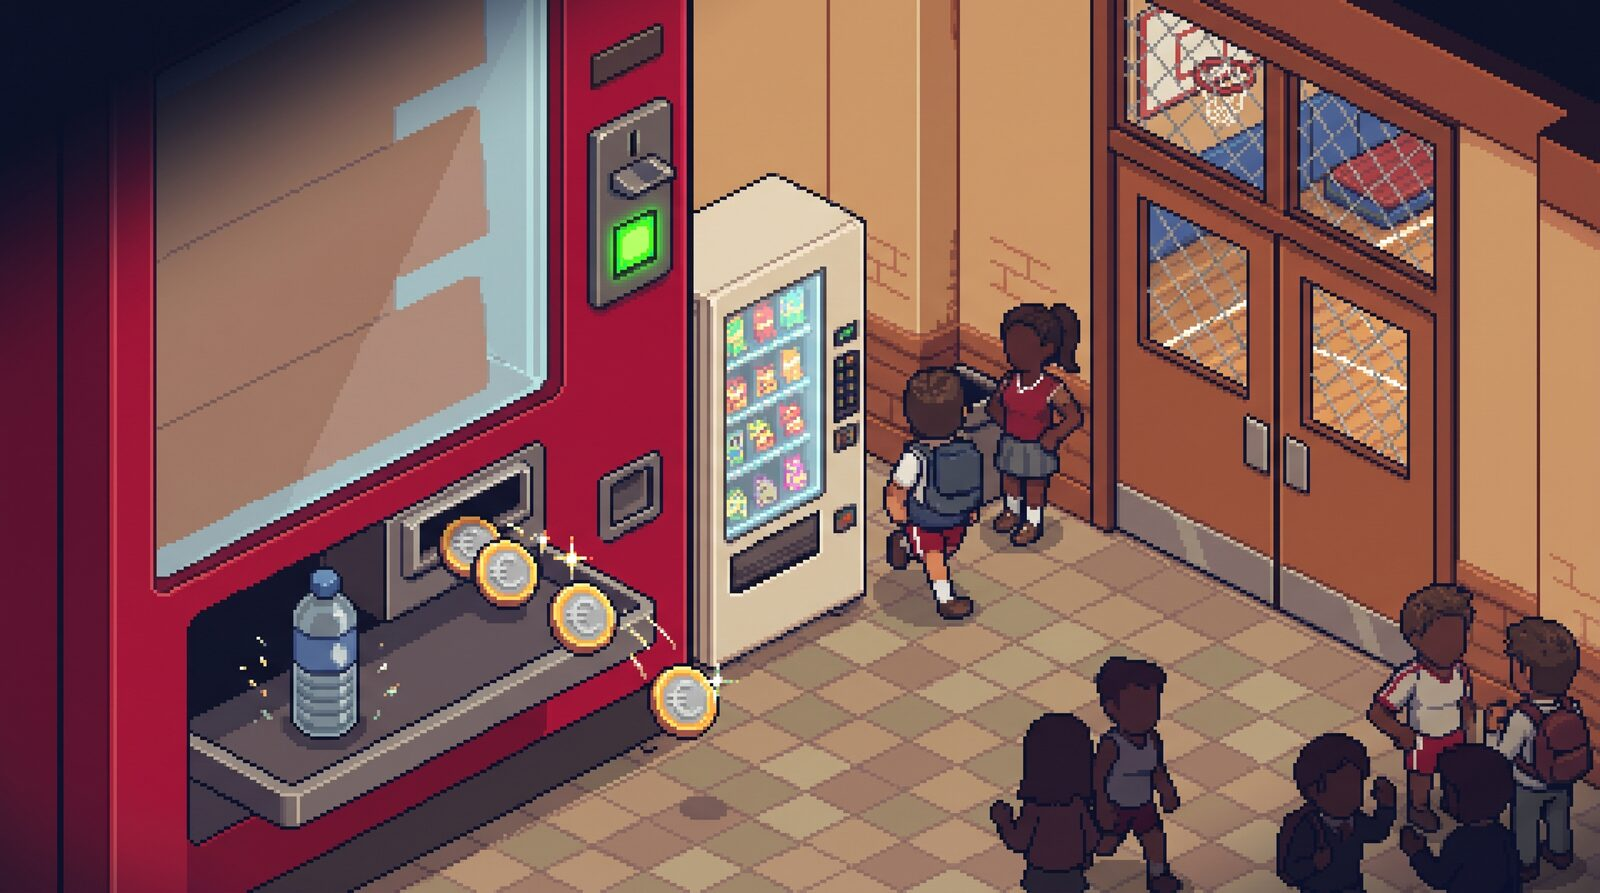
\includegraphics[width=0.8\textwidth]{../2026-10-12/presentazione/immagini/resto.jpeg}
\end{center}

\begin{esempio}[La Richiesta di Marta]
\textbf{Da:} Marta, responsabile distributori \textbullet{} \textbf{Oggetto:} distributore del piano terra

\smallskip
\emph{Ciao ragazzi! Sono Marta, gestisco i distributori del piano terra, quelli vicino alla palestra che all'intervallo delle 10:50 vengono presi d'assalto. Vorrei che la macchina, quando un cliente sceglie un prodotto, controllasse se il credito inserito è sufficiente. Se lo è, deve erogare il prodotto e restituire il resto; se non lo è, deve mostrare quanto manca. Per esempio: un cliente inserisce 2,00\,\euro{} e sceglie una bottiglietta d'acqua da 0,60\,\euro. Grazie mille e buona giornata!}
\end{esempio}

\begin{soluzione}[La Richiesta Annotata e la Scheda I-P-O]
\rumore{Ciao ragazzi! Sono Marta, gestisco i distributori del piano terra, quelli vicino alla palestra che all'intervallo delle 10:50 vengono presi d'assalto.} Vorrei che la macchina, quando un cliente sceglie un prodotto, controllasse \regola{se il credito inserito è sufficiente}\confronto{$\geq$}. Se lo è, deve \richiesta{erogare il prodotto e restituire il resto}; \regola{se non lo è}\confronto{$<$}, deve \richiesta{mostrare quanto manca}. Per esempio: un cliente inserisce \dato{2,00\,\euro} e sceglie una bottiglietta d'acqua da \dato{0,60\,\euro}. \rumore{Grazie mille e buona giornata!}

\begin{scheda}
Riformulo & \emph{``La macchina deve capire se il credito copre il prezzo e calcolare resto o importo mancante.''} \\ \hline
Input & credito = \textbf{2,00\,\euro} \textbullet{} prezzo = \textbf{0,60\,\euro} \\ \hline
Elaborazione & credito $\geq$ prezzo $\to$ resto = credito $-$ prezzo \newline altrimenti $\to$ mancano = prezzo $-$ credito \\ \hline
Output & prodotto + resto \textbf{oppure} ``Mancano X\,\euro'' \\ \hline
Prova a mano & $2{,}00 \geq 0{,}60$ \textbf{VERO} $\to$ resto $2{,}00 - 0{,}60$ = \textbf{1,40\,\euro} \newline Caso limite: credito 0,60\,\euro{} $\to$ eroga, resto 0,00\,\euro \\ \hline
Domande & ? E se il prodotto è \textbf{esaurito}? La richiesta non lo dice. \\ \hline
\end{scheda}
\end{soluzione}

% ==============================================================================
\newpage
\section{Le 5 Richieste di Marta}
% ==============================================================================

Modalità: \textbf{a coppie}. Su ogni richiesta evidenzia con colori o simboli. Sul quaderno scrivi la frase \emph{``La macchina deve\dots''}, la scheda I-P-O, la prova a mano e \textbf{almeno una domanda per Marta}.

\begin{esercizio}[Richiesta 1: Bicchierini Esauriti]
Ciao, sono ancora Marta. Il distributore delle bevande calde del primo piano è un modello vecchiotto, grigio, comprato nel 2019, e il caffè lungo è il preferito della prof di italiano. Ogni bicchierino costa alla scuola 5 centesimi e d'inverno ne usiamo circa 300 a settimana. Il problema è che, quando i bicchierini finiscono, la macchina versa lo stesso il caffè\dots{} direttamente nello scarico! Vorrei che, quando un cliente sceglie una bevanda, la macchina controllasse se c'è ancora almeno un bicchierino: se c'è, prepara la bevanda e i bicchierini diminuiscono di uno; se non c'è, non prepara niente e mostra ``Bicchieri esauriti''. Adesso nel tubo ci sono 40 bicchierini.
\end{esercizio}

\begin{esercizio}[Richiesta 2: La Gettoniera in Centesimi]
Ciao! Il tecnico della ditta, simpaticissimo, mi ha spiegato che la gettoniera nuova ragiona tutto in centesimi, mentre sul listino i prezzi sono scritti in euro. Le patatine costano 1,20\,\euro. Un cliente inserisce tre monete da 50 centesimi. La macchina deve restituire il resto usando soltanto monete da 10 centesimi. Il tecnico ha detto che ripasserà giovedì per controllare. Quante monete da 10 centesimi deve restituire la macchina?
\end{esercizio}

\begin{esercizio}[Richiesta 3: La Promo d'Autunno]
Buongiorno! Per festeggiare l'arrivo dell'autunno (e delle castagne!) lanciamo una promozione. Chi inserisce almeno 3\,\euro{} di credito riceve uno snack in omaggio; chi inserisce più di 5\,\euro{} riceve anche una bottiglietta d'acqua gratis. Attenzione: la promozione vale per tutti tranne chi paga con la chiavetta ricaricabile. Che omaggi spettano a un cliente che inserisce esattamente 5\,\euro{} in monete?
\end{esercizio}

\begin{esercizio}[Richiesta 4: L'Avviso di Rifornimento]
Ciao ragazzi, ultima richiesta della settimana, promesso! Ogni spirale della macchina snack contiene al massimo 12 prodotti. Vorrei che la macchina mi mandasse un avviso quando una spirale sta per finire, così il tecnico passa a riempirla prima che i ragazzi restino a bocca asciutta. Il tecnico di solito passa il martedì mattina. Ah, l'avviso deve arrivare anche quando una spirale è proprio vuota. Grazie!
\end{esercizio}

\begin{esercizio}[Richiesta 5: La Macchina del Secondo Piano]
Ciao a tutti! Dopo la riunione di ieri con il preside (due ore, che fatica!) abbiamo deciso: dalla prossima settimana la macchina snack del secondo piano accetterà solo monete da 50 centesimi, 1\,\euro{} e 2\,\euro. Il cliente inserisce le monete e digita il codice dello snack. Se lo snack è esaurito, la macchina restituisce tutte le monete inserite. Se invece è disponibile e il credito basta, eroga lo snack e dà il resto. Se il credito non basta, aspetta altre monete. Esempio: un cliente inserisce una moneta da 1\,\euro{} e una da 50 centesimi e digita B2, i cracker, che costano 1,30\,\euro. Nella spirale B2 ne restano 4.
\end{esercizio}

\begin{consiglio}[La Scheda I-P-O da Copiare sul Quaderno]
\begin{scheda}
Riformulo & La macchina deve \dotfill \\ \hline
Input & (nome = valore + unità) \\ \hline
Elaborazione & (calcoli e confronti) \\ \hline
Output & \\ \hline
Prova a mano & (+ caso limite) \\ \hline
Domande & (per il cliente) \\ \hline
\end{scheda}
\end{consiglio}

% ==============================================================================
\newpage
\section{Soluzioni Commentate}
% ==============================================================================

\begin{soluzione}[Richiesta 1: Bicchierini Esauriti --- trappola: il rumore]
\rumore{Ciao, sono ancora Marta. Il distributore delle bevande calde del primo piano è un modello vecchiotto, grigio, comprato nel 2019, e il caffè lungo è il preferito della prof di italiano. Ogni bicchierino costa alla scuola 5 centesimi e d'inverno ne usiamo circa 300 a settimana. Il problema è che, quando i bicchierini finiscono, la macchina versa lo stesso il caffè\dots{} direttamente nello scarico!} Vorrei che, quando un cliente sceglie una bevanda, la macchina controllasse \regola{se c'è ancora almeno un bicchierino}\confronto{$\geq$ 1}: se c'è, \richiesta{prepara la bevanda e i bicchierini diminuiscono di uno}; \regola{se non c'è}\confronto{= 0}, \richiesta{non prepara niente e mostra ``Bicchieri esauriti''}. Adesso nel tubo ci sono \dato{40 bicchierini}.

\begin{scheda}
Riformulo & \emph{``Prima di preparare, la macchina deve controllare che ci sia almeno un bicchierino.''} \\ \hline
Input & bicchierini nel tubo = \textbf{40} \textbullet{} bevanda scelta \\ \hline
Elaborazione & ``almeno uno'' $\to$ bicchierini $\geq$ 1 \newline se sì: i bicchierini scendono di 1 \\ \hline
Output & bevanda + bicchierini aggiornati \textbf{oppure} ``Bicchieri esauriti'' \\ \hline
Prova a mano & $40 \geq 1$ \textbf{VERO} $\to$ bevanda, ne restano 39. \newline Caso limite: 1 bicchierino $\to$ prepara, ne restano 0. \\ \hline
Domande & ? Se i bicchieri sono esauriti, le \textbf{monete inserite} vengono restituite? \\ \hline
\end{scheda}
Lo sfogo sul caffè nello scarico spiega il \emph{perché} della richiesta, ma non entra nella scheda. Anche i 5 centesimi e i 300 bicchieri sono numeri esca.
\end{soluzione}

\begin{soluzione}[Richiesta 2: La Gettoniera in Centesimi --- trappole: dato nascosto e unità]
Ciao! \rumore{Il tecnico della ditta, simpaticissimo, mi ha spiegato che} la gettoniera nuova \regola{ragiona tutto in centesimi}\nascosto{1\,\euro{} = 100 cent}, mentre sul listino i prezzi sono scritti in euro. Le patatine costano \dato{1,20\,\euro}. Un cliente inserisce \dato{tre monete da 50 cent}\calcolo{credito = 3 $\times$ 50}. La macchina deve restituire il resto \regola{usando soltanto monete da} \dato{10 centesimi}. \rumore{Il tecnico ha detto che ripasserà giovedì per controllare.} \richiesta{Quante monete da 10 centesimi deve restituire la macchina?}

\begin{scheda}
Riformulo & \emph{``La macchina deve calcolare il resto in centesimi e contare le monete da 10.''} \\ \hline
Input & prezzo = \textbf{1,20\,\euro} \textbullet{} monete = \textbf{3 da 50 cent} \newline taglio del resto = \textbf{10 cent} \textbullet{} $\bigstar$ 1\,\euro{} = \textbf{100 cent} \\ \hline
Elaborazione & tutto in centesimi: prezzo = 120, credito = $3 \times 50 = 150$ \newline resto = credito $-$ prezzo \textbullet{} monete = resto $\div$ 10 \\ \hline
Output & numero di monete da 10 centesimi \\ \hline
Prova a mano & $150 - 120 = 30$ cent $\to$ $30 \div 10$ = \textbf{3 monete}. \newline Errore tipico: $1{,}50 - 120$ = numero negativo! \\ \hline
Domande & ? E se il resto non è un multiplo di 10 (prezzo 1,25\,\euro)? \\ \hline
\end{scheda}
\end{soluzione}

\begin{soluzione}[Richiesta 3: La Promo d'Autunno --- trappola: le parole-trappola]
\rumore{Buongiorno! Per festeggiare l'arrivo dell'autunno (e delle castagne!)} lanciamo una promozione. Chi inserisce \regola{almeno}\confronto{$\geq$} \dato{3\,\euro} di credito riceve \richiesta{uno snack in omaggio}; chi inserisce \regola{più di}\confronto{$>$} \dato{5\,\euro} riceve anche \richiesta{una bottiglietta d'acqua gratis}. Attenzione: la promozione vale per tutti \regola{tranne chi paga con la chiavetta ricaricabile}\confronto{$\neq$}. \richiesta{Che omaggi spettano} a un cliente che inserisce \dato{esattamente 5\,\euro} \dato{in monete}?

\begin{scheda}
Riformulo & \emph{``La macchina deve decidere gli omaggi in base al credito e a come si paga.''} \\ \hline
Input & credito = \textbf{5,00\,\euro} \textbullet{} pagamento = \textbf{monete} \newline soglie: \textbf{3\,\euro} (snack) e \textbf{5\,\euro} (acqua) \\ \hline
Elaborazione & prima: pagamento $\neq$ chiavetta \newline snack se credito $\geq$ 3 \textbullet{} acqua se credito $>$ 5 \\ \hline
Output & nessun omaggio / solo snack / snack + acqua \\ \hline
Prova a mano & $5 \geq 3$ \textbf{VERO} $\to$ snack \textbullet{} $5 > 5$ \textbf{FALSO} $\to$ niente acqua. \newline Risposta: \textbf{solo lo snack}. Con la chiavetta: nessun omaggio. \\ \hline
Domande & ? Vale una volta sola per cliente? Fino a quando dura la promo? Marta voleva davvero escludere i 5\,\euro{} esatti dall'acqua? \\ \hline
\end{scheda}
\end{soluzione}

\begin{soluzione}[Richiesta 4: L'Avviso di Rifornimento --- trappola: i dati mancanti]
\rumore{Ciao ragazzi, ultima richiesta della settimana, promesso!} Ogni spirale della macchina snack contiene \regola{al massimo}\confronto{$\leq$} \dato{12 prodotti}. Vorrei che la macchina mi mandasse \richiesta{un avviso}\mancante{come e a chi?} \regola{quando una spirale sta per finire}\mancante{quanti pezzi?}, \rumore{così il tecnico passa a riempirla prima che i ragazzi restino a bocca asciutta. Il tecnico di solito passa il martedì mattina.} Ah, l'avviso deve arrivare \regola{anche quando una spirale è proprio vuota}\confronto{= 0}. \rumore{Grazie!}

\begin{scheda}
Riformulo & \emph{``La macchina deve avvisare quando i prodotti di una spirale scendono a una certa soglia.''} \\ \hline
Input & prodotti in ogni spirale \textbullet{} capienza = \textbf{12} \newline soglia = \textbf{? MANCA} \\ \hline
Elaborazione & per ogni spirale: prodotti $\leq$ soglia $\to$ avviso \newline (la spirale vuota, 0, è già compresa) \\ \hline
Output & avviso al gestore con la spirale da riempire \\ \hline
Prova a mano & Impossibile senza soglia! Se fosse 3: spirale con 3 $\to$ $3 \leq 3$ $\to$ avviso. \\ \hline
Domande & ? Quanti pezzi significa ``sta per finire''? \newline ? Avviso via email, SMS o display? Un avviso per spirale o uno riassuntivo? \\ \hline
\end{scheda}
La capienza di 12 non serve all'avviso, ma servirà al tecnico: non è rumore, è un dato per un'altra funzione.
\end{soluzione}

\begin{soluzione}[Richiesta 5: La Macchina del Secondo Piano --- tutte le trappole]
\rumore{Ciao a tutti! Dopo la riunione di ieri con il preside (due ore, che fatica!) abbiamo deciso: dalla prossima settimana} la macchina snack \rumore{del secondo piano} \regola{accetterà solo monete da 50 centesimi, 1\,\euro{} e 2\,\euro}. Il cliente inserisce le monete e digita il codice dello snack. \regola{Se lo snack è esaurito}\confronto{= 0}, la macchina \richiesta{restituisce tutte le monete inserite}. \regola{Se invece è disponibile e il credito basta}\confronto{$\geq$}, \richiesta{eroga lo snack e dà il resto}. \regola{Se il credito non basta}\confronto{$<$}, \richiesta{aspetta altre monete}\mancante{quanto?}. Esempio: un cliente inserisce \dato{una moneta da 1\,\euro} \dato{e una da 50 centesimi}\nascosto{credito 1,50\,\euro} e digita \dato{B2}, \rumore{i cracker,} che costano \dato{1,30\,\euro}. Nella spirale B2 ne restano \dato{4}.

\begin{scheda}
Riformulo & \emph{``La macchina deve scegliere tra 3 strade: rimborso, snack con resto, attesa.''} \\ \hline
Input & $\bigstar$ credito = 1 + 0,50 = \textbf{1,50\,\euro} \textbullet{} codice = \textbf{B2} \newline prezzo B2 = \textbf{1,30\,\euro} \textbullet{} quantità B2 = \textbf{4} \\ \hline
Elaborazione & 1. quantità = 0 $\to$ rimborso \newline 2. credito $\geq$ prezzo $\to$ snack + resto (credito $-$ prezzo) \newline 3. altrimenti $\to$ attesa \\ \hline
Output & rimborso / snack + resto / attesa di altre monete \\ \hline
Prova a mano & $4 \neq 0$ $\to$ disponibile \textbullet{} $1{,}50 \geq 1{,}30$ \textbf{VERO} $\to$ snack + resto \textbf{0,20\,\euro} \\ \hline
Domande & ? Per quanto tempo aspetta? \textbullet{} ? Una moneta da 20 cent viene rifiutata o tenuta? \newline ? E se in cassa non ci sono monete per il resto? \\ \hline
\end{scheda}
L'ordine delle regole conta: si controlla prima la disponibilità, poi il credito.
\end{soluzione}

% ==============================================================================
\section{Errori Tipici e Checklist dell'Analista}
% ==============================================================================

\begin{attenzione}[Gli Errori Più Comuni]
\begin{itemize}
  \item Usare tutti i numeri del messaggio (anche il 2019).
  \item Mescolare euro e centesimi nello stesso calcolo.
  \item Leggere ``almeno'' come ``più di'' (e viceversa).
  \item Inventare la soglia invece di chiederla.
  \item Dimenticare i casi che il cliente non ha scritto.
\end{itemize}
\end{attenzione}

\begin{consiglio}[Il Controllo Qualità di Ogni Nuova Funzione]
\begin{itemize}
  \item[$\square$] Ho letto la richiesta \textbf{due volte}?
  \item[$\square$] Ho \textbf{barrato} il rumore, anche i numeri che non servono?
  \item[$\square$] Ogni dato ha \textbf{nome, valore e unità di misura}?
  \item[$\square$] Ho cercato i \textbf{dati nascosti} ($\bigstar$) e quelli \textbf{mancanti} (?)?
  \item[$\square$] Ho tradotto le regole in \textbf{confronti} ($\geq$, $>$, $\leq$, $<$, $=$, $\neq$)?
  \item[$\square$] Ho provato il \textbf{caso limite}?
  \item[$\square$] Ho scritto le \textbf{domande per il cliente}?
\end{itemize}
\end{consiglio}

\begin{esercizio}[Biglietto d'Uscita: La Spia del Frigo]
Il frigorifero della macchina delle bibite deve accendere la spia di manutenzione se la temperatura interna supera gli 8 gradi. Il frigorifero è stato pulito martedì dal tecnico. In questo momento il termometro segna 8 gradi. La spia si accende?
\end{esercizio}

\begin{soluzione}[Biglietto d'Uscita: La Spia del Frigo]
Il frigorifero della macchina delle bibite deve \richiesta{accendere la spia di manutenzione} \regola{se la temperatura interna supera}\confronto{$>$} gli \dato{8 gradi}. \rumore{Il frigorifero è stato pulito martedì dal tecnico.} In questo momento il termometro segna \dato{8 gradi}. \richiesta{La spia si accende?}

\begin{scheda}
Riformulo & \emph{``La macchina deve accendere la spia solo se fa più caldo di 8 gradi.''} \\ \hline
Input & temperatura = \textbf{8 gradi} \textbullet{} soglia = \textbf{8 gradi} \\ \hline
Elaborazione & ``supera'' $\to$ temperatura $>$ 8 \\ \hline
Output & spia accesa \textbf{oppure} spia spenta \\ \hline
Prova a mano & $8 > 8$ \textbf{FALSO} $\to$ la spia resta \textbf{spenta}. \\ \hline
Domande & ? Con 8 gradi esatti Marta vuole davvero la spia spenta? \\ \hline
\end{scheda}
\end{soluzione}


% \part{La Programmazione Orientata agli Oggetti (OOP)}
% \input{capitoli/04_classi_e_oggetti}
% \input{capitoli/05_incapsulamento_e_metodi}
% \input{capitoli/06_ereditarieta_e_polimorfismo}

% \part{Strutture Dati e Persistenza}
% \input{capitoli/07_collezioni_avanzate}
% \input{capitoli/08_file_json_e_csv}
% \input{capitoli/09_gestione_eccezioni}

% \part{Progetto Software Annuale}
% \input{capitoli/10_architettura_progetto}
% \input{capitoli/11_rilascio_e_documentazione}

% ==============================================================================
% PARTE CONCLUSIVA (BACKMATTER)
% ==============================================================================
\backmatter

\chapter{Riferimento Rapido e Cheat-Sheet}
\noindent Tavole sinottiche di riferimento rapido per le convenzioni di codice, comandi Git di frequente utilizzo e pattern di progettazione.

\section*{Il Kit dell'Analista}
\begin{center}
\renewcommand{\arraystretch}{1.45}
\begin{tabular}{|l|l|l|}
\hline
\rowcolor{PiazzaPrimary!15}
\textbf{Cosa cerco} & \textbf{Come appare} & \textbf{Simbolo a mano} \\
\hline
Dato            & \dato{1,30\,\euro}            & cerchio \\
Richiesta       & \richiesta{dà il resto}       & doppia sottolineatura \\
Regola          & \regola{se il credito basta}  & onda \\
Rumore          & \rumore{il tecnico del martedì} & barrato \\
Dato nascosto   & \nascosto{1\,\euro{} = 100 cent} & $\bigstar$ a margine \\
Dato mancante   & \mancante{quanti pezzi?}      & ? a margine + domanda per il cliente \\
\hline
\end{tabular}
\end{center}

\section*{Parole che Diventano Confronti}
\begin{center}
\renewcommand{\arraystretch}{1.3}
\begin{tabular}{|l|c||l|c|}
\hline
\rowcolor{PiazzaPrimary!15}
\textbf{Parola} & \textbf{Confronto} & \textbf{Parola} & \textbf{Confronto} \\
\hline
almeno, basta       & $\geq$ & più di, supera      & $>$ \\
al massimo, fino a  & $\leq$ & meno di, sotto      & $<$ \\
esattamente, pari a & $=$    & diverso da, tranne  & $\neq$ \\
\hline
\end{tabular}
\end{center}

\section*{La Scheda dei Requisiti}
\noindent Riformulo (\emph{``La macchina deve\dots''}) $\to$ Input (nome, valore, unità) $\to$ Elaborazione $\to$ Output $\to$ Prova a mano con caso limite $\to$ Domande per il cliente.

\end{document}
